\documentclass[12pt,a4paper]{article}
% This text is inserted in the beginning of all
% LaTex and Tex files I create.
%
% File created: Tue Sep 26 2017
% File name:    report_template.tex
% Path:         /home/name/Classes/AMPIII/Template/
%
% Name
% Sept, 2017
%

%recommended by fancyhdr package
\setlength{\headheight}{14.49998pt}
\addtolength{\topmargin}{-2.49998pt}

% include a minimal set of useful packages
\usepackage{graphicx}
\usepackage{amsfonts} 
\usepackage{amssymb}
\usepackage{amsmath}
\usepackage[a4paper,margin=4cm]{geometry}
\usepackage{lastpage}
\usepackage{fancyhdr}
\usepackage{hyperref}

\newcommand{\titlestr}{Security Analysis of Large-Scale Computer Systems}
\newcommand{\shorttitlestr}{EP2790 HT22 (50475)}
\newcommand{\authorstr}{Dairon Andrés Benites Aldaz} 

\begin{document}
%%%%%%%%%%%%%%%%%%%%%%%%%%%%%%555
% title page
\begin{titlepage}
  \centering
  
  {\LARGE \titlestr }

  \vspace{1cm}
  {\Large \authorstr \par}

  {\bf \href{mailto:daba2@kth.se}{daba2@kth.se}}

  \vspace{1cm}
  \today     % PUT YOUR DATE HERE
  
  \vspace{2cm}


  
\includegraphics[width=0.35\textwidth]{figures/logo.png}
  

  \vspace{2cm}
  \flushleft
  
  Project Area: {\bf IT Security } \\
  Project Supervisor \\ {\bf Ashish Kumar Dwivedi, Mathias Ekstedt \& Zeeshan Afzal } \\

  \vspace{5mm} {\footnotesize In submitting this work I am indicating
    that I have read the KTH's Academic Integrity Policy. I
    declare that all material in this assessment is my own work except
    where there is clear acknowledgement and reference to the work of
    others.\par}
  \vfill
\end{titlepage}

% put headings on each page
\pagestyle{fancy}
\fancyhf{}
\rhead{\shorttitlestr}
\lhead{\authorstr}
\rfoot{Page \thepage\ of \pageref{LastPage}}
\renewcommand{\headrulewidth}{1pt}

%%%%%%%%%%%%%%%%%%%%%%%%%%%%%%555
\section{Security Analysis of one of the largest Bitcoin Exchange Platform}
\subsection{Background}
\begin{quote}
"Security isn’t something you buy, it’s something you do, and it takes talented people to do it right"
\end{quote}
\begin{justify}
\subsubsection{Coinbase Global, Inc.}
Being an all American publicly traded firm, \textit{Coinbase®} works mainly as a bitcoin exchange platform. Most of their employees work remotely, and the business has no physical headquarters. By trading volume, it is the biggest cryptocurrency exchange in the US. Brian Armstrong and Fred Ehrsam launched the business in 2012. As part of a wave of numerous significant tech businesses closing headquarters in San Francisco following the COVID-19 epidemic, Coinbase announced in May 2020 that it would close its San Francisco, California headquarters and transition to a \textbf{remote-first model}.
\end{justify}
 \subsubsection{The good}
 \begin{justify}
Coinbase has been know to implement quite a number of interesting security features. They pride on calling themselves \textbf{"The most trusted crypto exchange"} as of the time of this writing they have more than 103 million users trusting their services. They offer 2-Step Verification on all accounts, password management and even machine learning models that evaluate crypto-transactions in order to cancel a transaction before it is submitted if it does not look quite right.
 \end{justify}
  \subsubsection{The bad}
 \begin{justify}
There have been several attacks that have raised concern among some users, to mention a few: in January 2019, they stopped all trading on \textbf{Ethereum} since there have been some signs of an attack on the network. After this incident, it has been known that they have acquired via absortion an Italian startup called \textit{Neutrino}. They offered a \textit{"blockchain intelligence platform"} even though their founders where actually related to the \textbf{Hacking Team} who have several claims of providing advanced internet surveillance technology to dictatorial governments.
 \end{justify}
 \clearpage
  \subsubsection{The ugly}
 \begin{justify}
Coinbase revealed in August that a \textbf{sophisticated hacking attack attempt} had been made against them in mid-June. \\
This alleged attack made use of two Firefox browser zero-day vulnerabilities as well as :
\begin{itemize}
    \item Spear-phishing and Social engineering techniques
    \footnote{Such as sending bogus emails from hijacked email accounts and building a fake landing page from the University of Cambridge}
        
    
\end{itemize}
One of the Firefox flaws (CVE-2019-11707) could let an attacker increase their level of  JavaScript access on a browser page, and the other could let them get out of the browser sandbox and run code on the host PC (CVE-2019–11708). The network was not breached, and no cryptocurrency was stolen thanks to the security team at Coinbase's detection and blocking of the attempt.
 \end{justify}
\section{Main technical components}
The main technical components of the "Coinbase environment" can be described as the elements needed to provide a certain level of service that gives user the capability to \textbf{buy, store and trade} different cryptocurrencies. (Mainly Bitcoin, Ethereum and Litecoin)
\subsubsection{Products}
\begin{justify}
For most of the products shown in Figure 1 Coinbase offers an \textbf{}API( Application Programming Interface) for other developers and merchants to accept payments.
\end{justify}
\begin{center}
    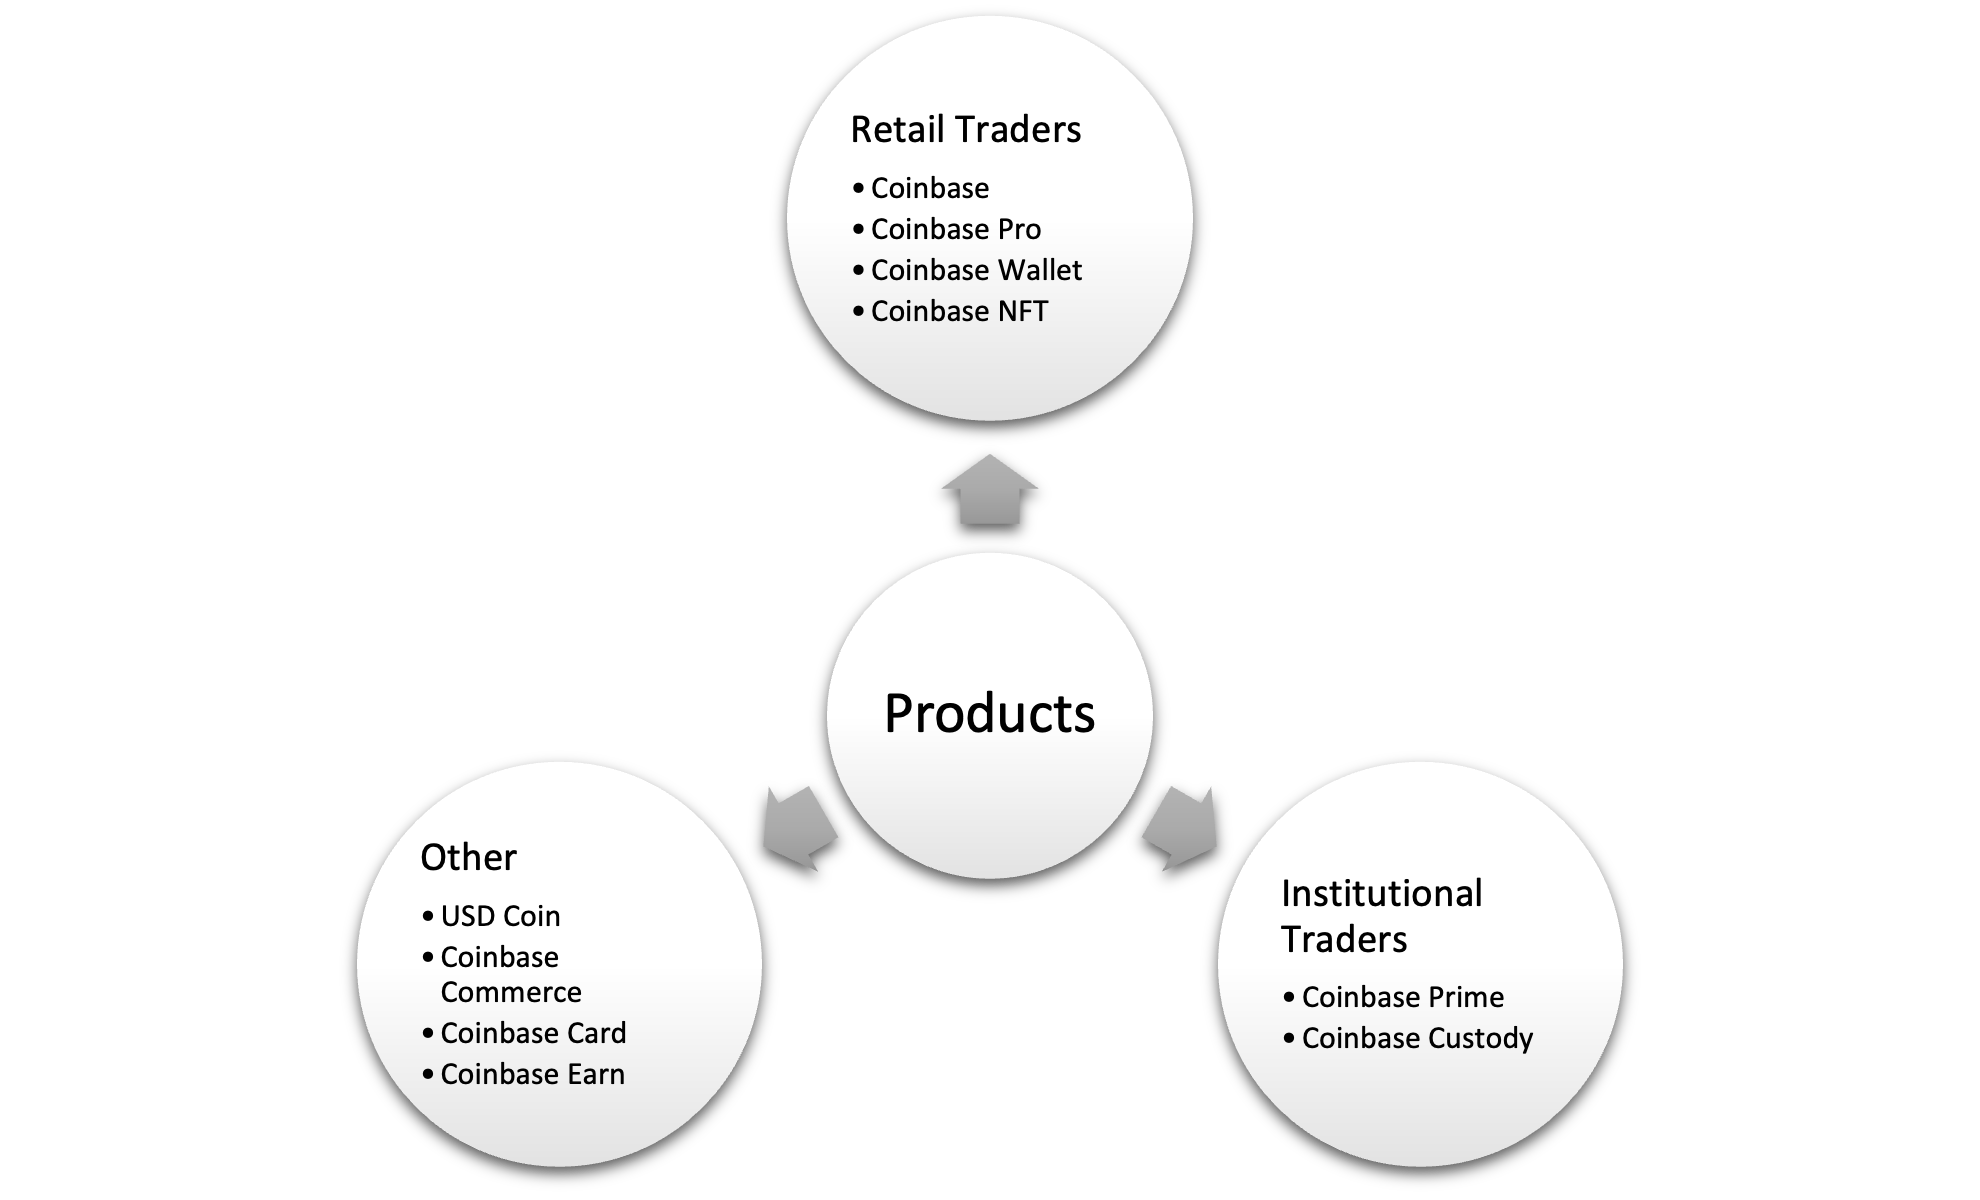
\includegraphics[width=0.85\textwidth]{figures/Picture 1.png}    
\end{center}
\subsubsection{Web}
Some of the elements mentioned above (and specially the ones that concern Coinbase Wallet®) are based on\textbf{ Web 3.0}.
This is a concept for public-blockchain based decentralised Internet.
We can make some distintions with prior \textit{popular} "standards":
\begin{center}
    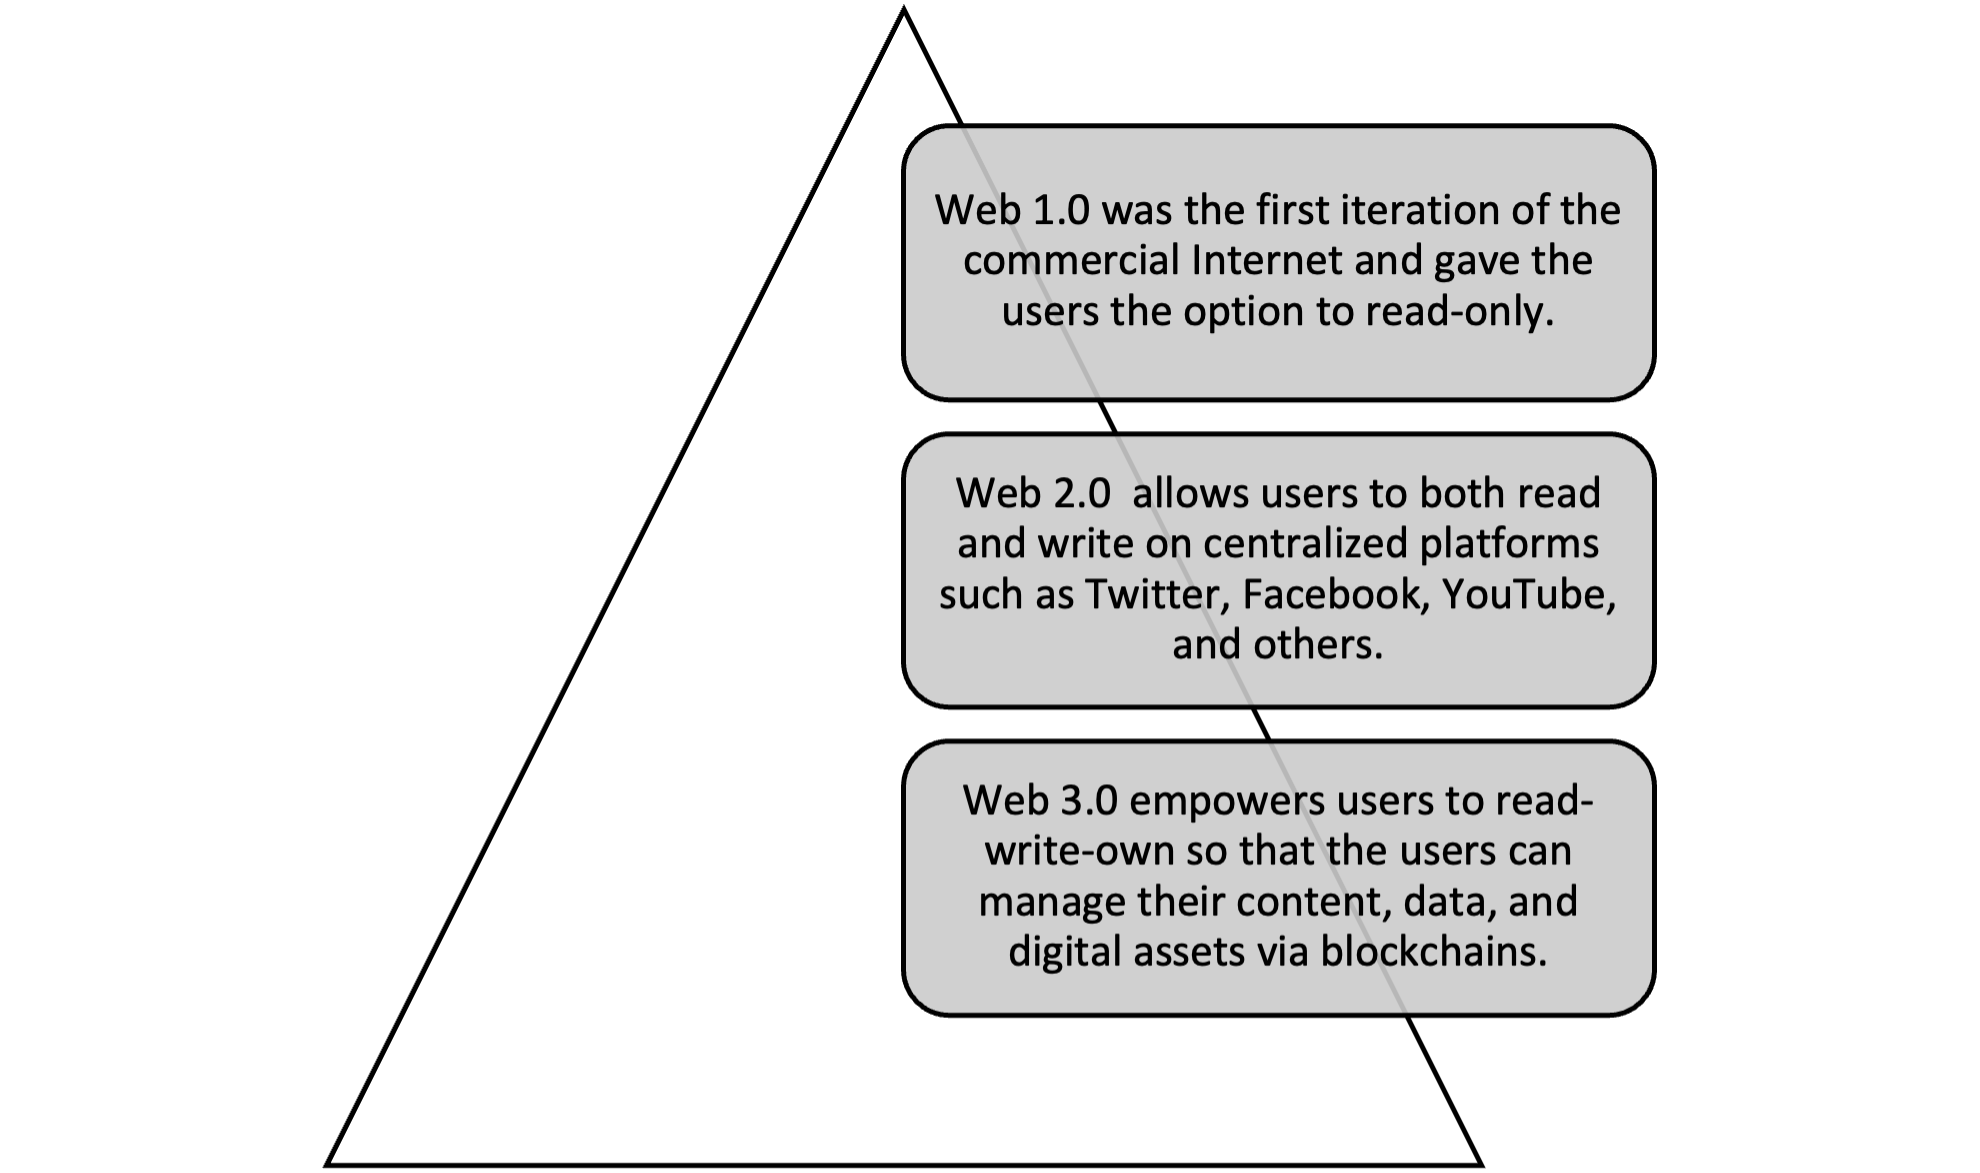
\includegraphics[width=0.85\textwidth]{figures/Picture2.png} 
\end{center}
\subsubsection{Infrastructure}
Most of Coinbase® services are provided through AWS (Amazon Web Services) since they cover most of their needs through some specific tools, such as: 
\begin{center}
    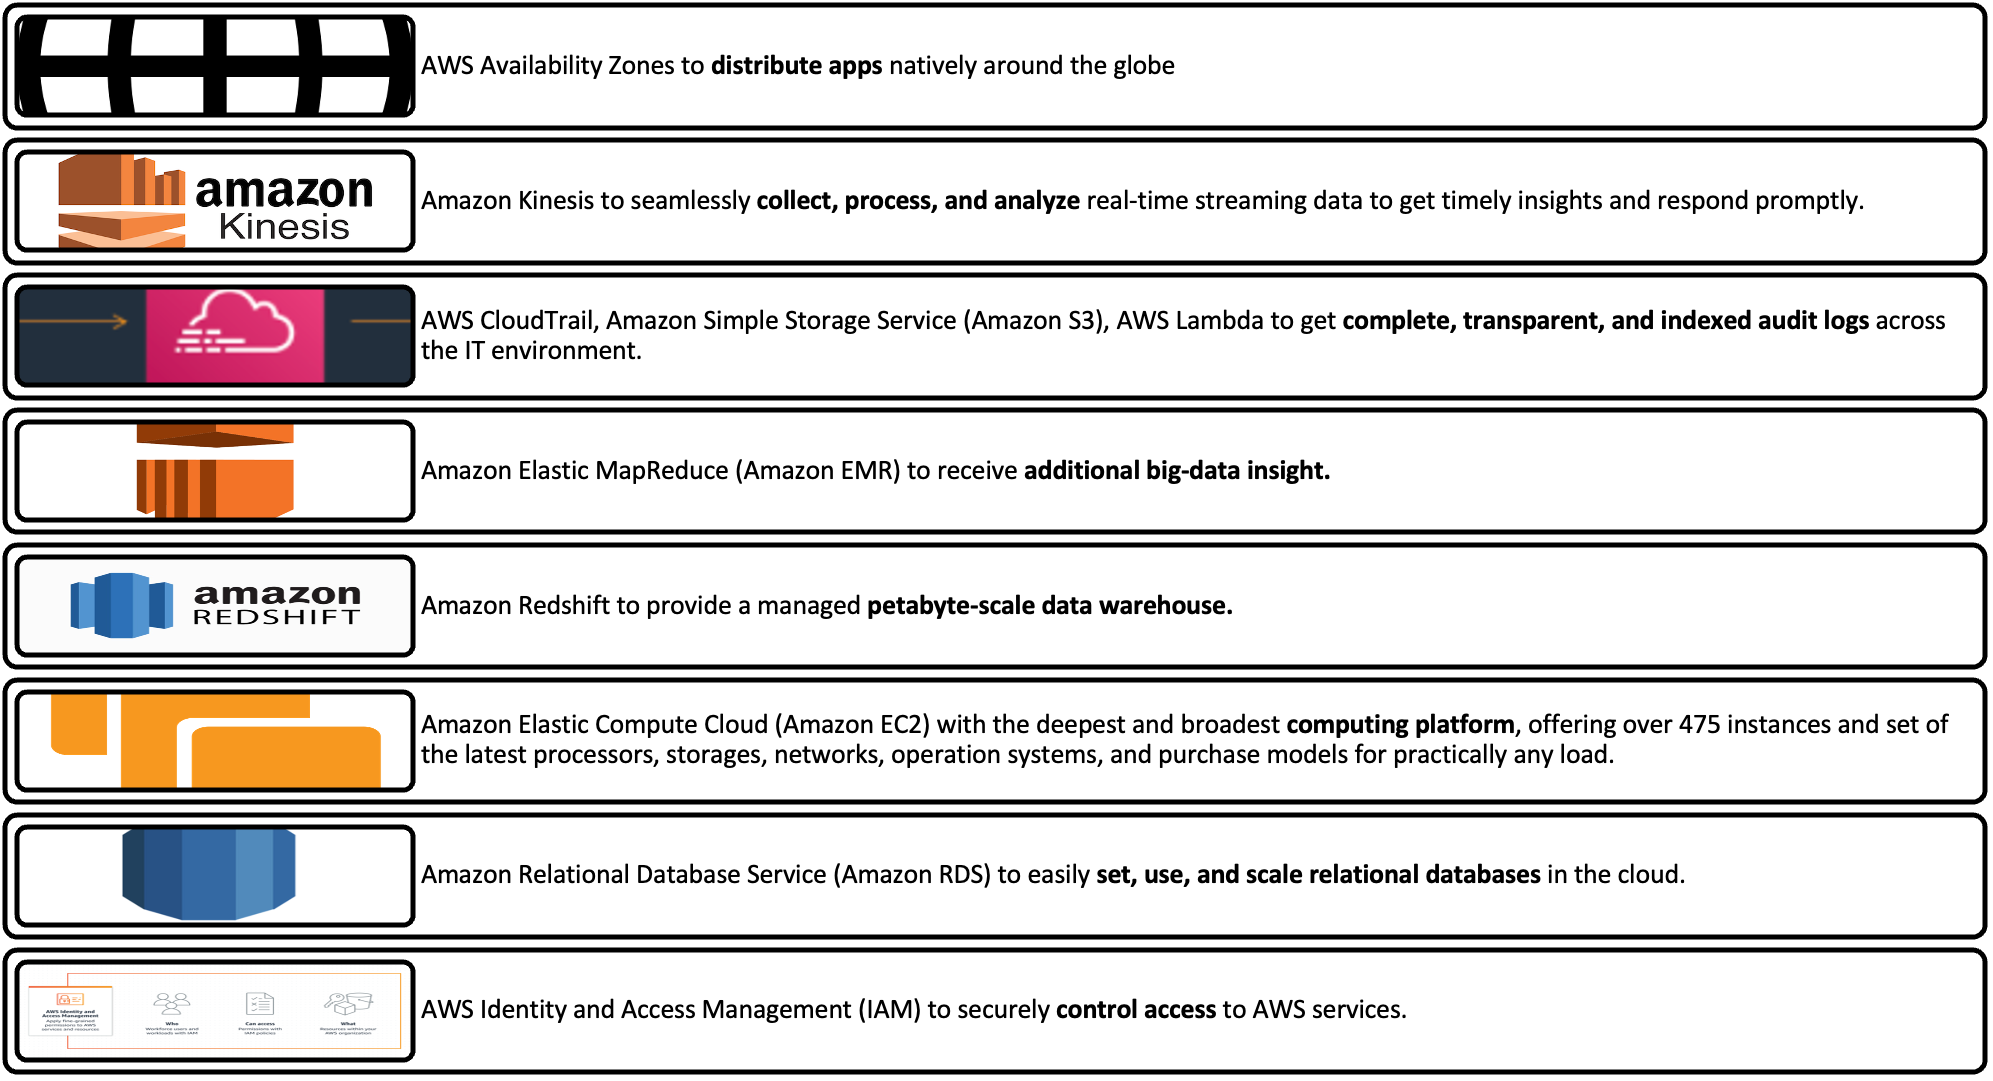
\includegraphics[width=0.85\textwidth]{figures/Picture3.png} 
\end{center}
\clearpage
\section{Purpose of the system}
The main purpose of the system can be defined as providing accessible and user-friendly experiences that make it easier to participate in decentralised finance\textbf{ (buy, sell and store \textit{crypto}) } while maintaining a high level of security.
Among other purposes of the system is to maintain a high level of service due to the scale of the deployment (Global). Protect customer privacy and segment based on the tax requirements of each region where they belong. Offer a platform where transaction security is prioritized.
\section{Delimitation}
A large part of the ecosystem to be analyzed will be based on the scenarios contemplated in recent years (post-pandemic) 2019 onwards. In addition, reference will be made to specific historical events within the world of cryptocurrencies since many of these threats are collective to the rest of the exchange providers.\\
With regard to threats, those that fall within the following areas will be considered:
\begin{enumerate}
    \item Social engineering
    \item Phishing
    \item Corporate Account Takeover (CATO)
    \item Distributed Denial of Service (DDoS) Attacks
    \item Ransomware
    \item Access to confidential information
    \item Identity theft
    \item Trashing
\end{enumerate} \\
Therefore, we will exclude from the list of possible threats scenarios related to the price variations of cryptocurrency products, threats related to the variation in the price of shares (convertible and non-convertible) belonging to or related to Coinbase Global, Inc.
 \clearpage
\bibliographystyle{plain}
\bibliography{bib_file}

\vspace{10mm}
\noindent \hrulefill

{\bf Notes:} 
None yet.


\end{document}


 